\section{Data and Methods}
\label{sec:data_methods}

\subsection{Hydrodynamic model}
\label{sec:methods_model}

Circulation was simulated with D-Flow Flexible Mesh (D-Flow FM, kernel
1.2.184) from the Delft3D FM Suite 2026.01, an unstructured finite-volume
solver for the three-dimensional shallow-water equations \citep{Kernkamp2011}.
The mesh of 25{,}212 faces covers the lagoon and an offshore extension to the
western Sicilian channel, over 11.96--12.56$^\circ$E and
37.70--38.06$^\circ$N, and grades from about 880~m offshore to about 60~m in
the lagoon and along the shorelines, so that about six cells span the North
Mouth. Ten sigma layers of uniform thickness, about 0.095~m at the mean depth
of 0.95~m, resolve the wind-driven surface drift over the near-bed return flow
reported by \citet{DeMarchis2012} and place the 0.40~m canopy of
Section~\ref{sec:methods_roughness} in the lowest four layers and part of the
fifth.

Turbulence closure used the $k$--$\varepsilon$ model, and density followed the
UNESCO equation of state with salinity and temperature as active constituents.
Bed roughness was a uniform Manning coefficient of 0.023~s~m$^{-1/3}$, the
solver default, standing for the bare substrate in every member, so that the
canopy is the only spatially variable resistance in the ensemble. Wind drag
followed the Charnock formulation with the coefficient taken from ERA5. The
simulation covered 1 to 10~July 2025 with an adaptive time step under a Courant
limit of 0.7, capped at 30~s in the members coupled to the wave model and at
15~s in the others, on eight MPI partitions (Supplementary Material,
Section~S1).

\subsection{Wave model and coupling}
\label{sec:methods_waves}

Waves were computed with SWAN \citep{Booij1999} through the Delft3D-WAVE
module, on an outer grid of $69 \times 54$ points at about 800~m and an inner
grid at about 90 by 110~m over the lagoon and its inlets, with
third-generation physics, depth-induced breaking \citep{BattjesJanssen1978} and
JONSWAP bottom friction. Flow and waves exchanged fields every 3600~s through
the DIMR framework, an interval set by the tidal and sea-breeze time scales,
and wave forces entered the flow as three-dimensional dissipation. Within each
exchange the wave model ran in stationary mode, which holds because wave energy
crosses the 2.5~km basin in about fifteen minutes (Section~S2 and Table~S1).
Where the canopy also entered the wave model, it did so through the vegetation
dissipation of \citet{Dalrymple1984} as implemented in SWAN by
\citet{Suzuki2012}, with the canopy parameters of the flow model averaged onto
the inner grid.

\subsection{Boundary and atmospheric forcing}
\label{sec:methods_forcing}

Open-sea boundaries were forced with the CMEMS Mediterranean Sea products,
water level from the analysis and forecast system, whose sea surface height
carries the tide, and salinity, temperature and a depth-resolved advection
velocity from the physical reanalysis. The advection velocity was required for
stability in the deep offshore cells. Since the CMEMS sea surface height is an
anomaly about the model rest state rather than a geodetic level, a per-node
offset of $+0.449$~m, anchored on the Marettimo tide gauge over 384 days and
distributed along the boundary by the CMEMS mean dynamic topography, was added
to the water-level boundary, and its seasonal residual of about 0.07~m bounds
the accuracy of the reference level (Section~S3).

Wind, mean sea level pressure and the Charnock parameter were taken from ERA5,
the wind blended with the AltaVilaEst record, and evaporation was imposed as
negative rainfall. Salinity and temperature were relaxed towards the CMEMS
fields with a time scale of 10~days, whose effect inside the lagoon is
quantified in Section~S3. Outside the lagoon both were initialised with the
CMEMS depth profiles at the start time, from 25.8~$^\circ$C and 37.5 at the
surface to 16.2~$^\circ$C and 38.3 below 260~m, and the lagoon with a salinity
of 42 and the surface temperature of the profile.

\subsection{Seagrass canopy parametrisation}
\label{sec:methods_roughness}

The canopy was represented as a three-dimensional drag field resolved per sigma
layer over the vertical extent of the plants, so that a cell whose canopy fills
two fifths of the water column carries drag in the layers within that fraction
and none above it. Drag per unit volume follows the quadratic form
\citep{Nepf2012}, with a drag coefficient $C_D$, a frontal width $D$, an areal
density $m$ and a canopy height $h_v$. The canopy responds to the flow through
the bending model of the solver, which balances the moment of the drag about
the leaf base against that of buoyancy, set by the difference between the
densities of sea water and leaf (Table~\ref{tab:veg}), and reduces the vertical
extent of the drag to $h_v \cos\varphi$ for a bending angle $\varphi$.

The trachytope framework of the solver, in which vegetation enters as a
composite bed roughness \citep{Baptist2007}, was not adopted, since a roughness
term acts at the bed whereas the factorial separates a momentum sink
distributed through the part of the column the plants occupy. For the same
reason the Gauckler--Strickler coefficient of 20~m$^{1/3}$~s$^{-1}$ calibrated
for this lagoon by \citet{Ingrassia2024}, equivalent to a Manning coefficient
of 0.050~s~m$^{-1/3}$, is a bulk roughness of the vegetated basin, and used as
the bare-substrate roughness of a model that resolves the canopy it would count
the canopy twice.

Table~\ref{tab:veg} gives the values and their provenance, none of them fitted
to any observation used to evaluate the model. Densities are expressed per leaf,
the element that presents the frontal area, and the canopy height is the
deflected extent of the drag rather than the leaf length, taken within the
range of flume and large-scale measurements of the species (Section~S4).
Fractional cover from the classification multiplies the areal density alone,
and median cover is 0.685 for \emph{P.\ oceanica} and 0.181 for
\emph{C.\ nodosa}, which therefore carries about 1.5\% of the total canopy
frontal area.

\begin{table}[H]
  \centering
  \caption{Canopy parameters. \emph{P.\ oceanica} values are from
  \citet{CiraoloFerreri2006}, except the canopy height, which is from
  \citet{Prinos2010}. \emph{C.\ nodosa} values are from \citet{Morris2008},
  with the shoot density also bracketed by \citet{Cancemi2002}.}
  \label{tab:veg}
  \begin{tabular}{lrr}
    \toprule
    Parameter & \emph{P.\ oceanica} & \emph{C.\ nodosa} \\
    \midrule
    Shoot density (m$^{-2}$)      & 500   & 800   \\
    Leaves per shoot              & 6     & 3     \\
    Leaf width $D$ (m)            & 0.010 & 0.004 \\
    Canopy height $h_v$ (m)       & 0.40  & 0.15  \\
    Leaf density (kg~m$^{-3}$)    & 900   & 900   \\
    Drag coefficient $C_D$        & 0.8   & 0.8   \\
    \bottomrule
  \end{tabular}
\end{table}

The classes were assigned from a supervised random-forest classification of
PlanetScope SuperDove imagery acquired in August 2023 at 3~m ground sampling
distance, following the depth-invariant approach of \citet{Maltese2025}, and
classified pixels were transferred to the flow links of the mesh, a link
straddling more than one class carrying each weighted by the area it occupies
(Figure~\ref{fig:seagrass}, Section~S4).

\begin{figure}[H]
  \centering
  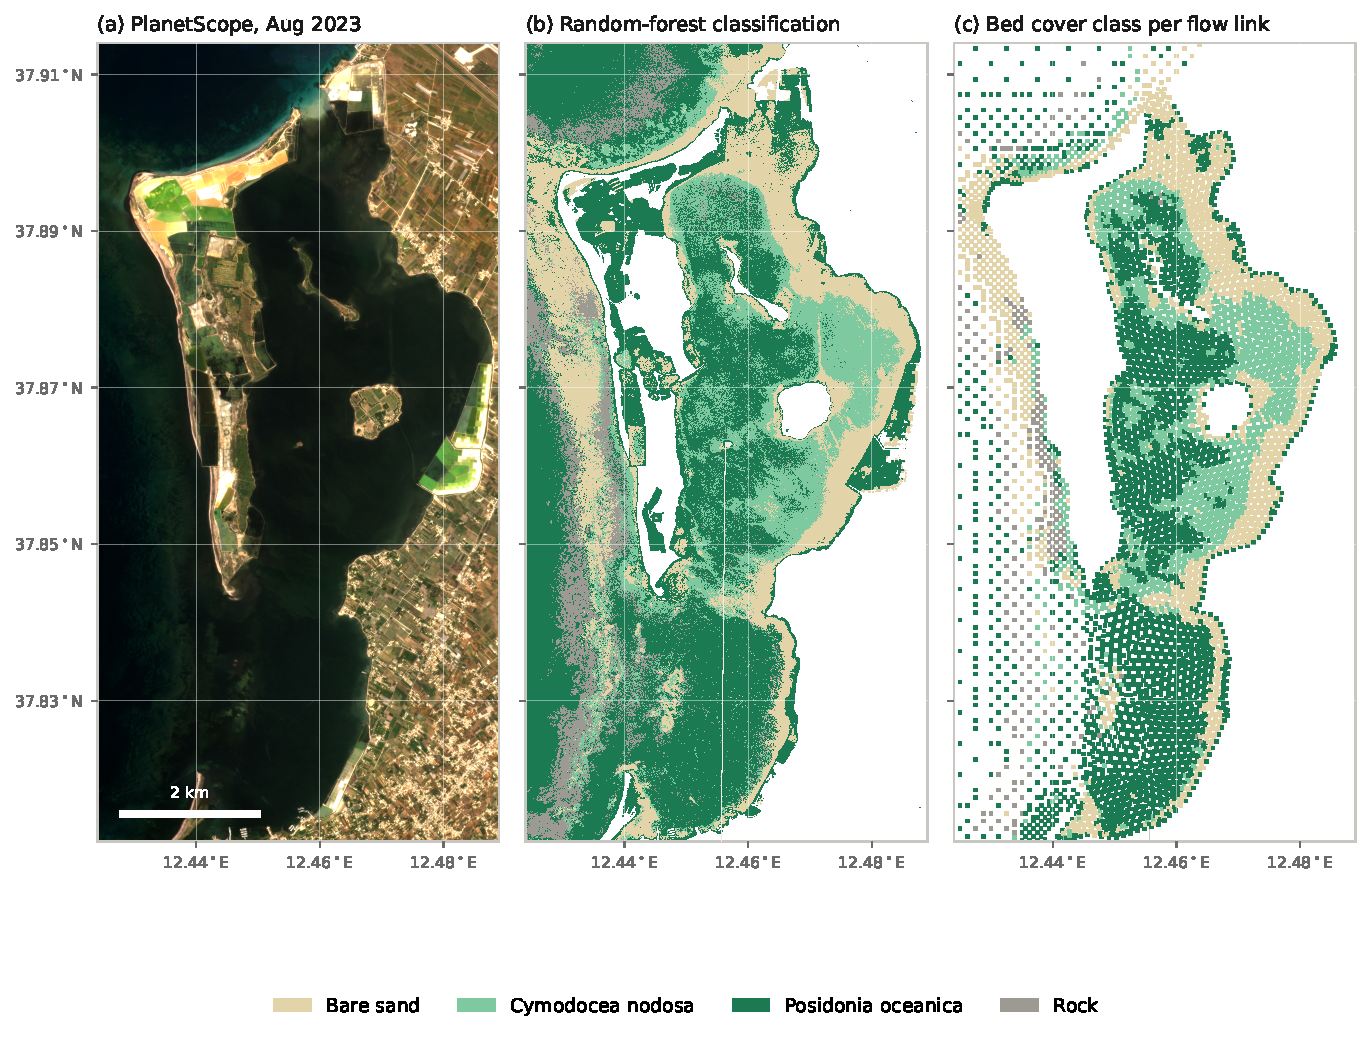
\includegraphics[width=\textwidth]{seagrass_classification}
  \caption{The seagrass map from imagery to model input. (a) PlanetScope
  SuperDove August 2023 median composite. (b) The random-forest classification,
  with the six output classes collapsed to the four seagrass classes. (c) The
  dominant bed cover class at each flow link, from the classification file the
  model reads, at the mesh resolution onto which the classification is
  sampled. The classification is computed over the whole scene, but only links
  inside the lagoon carry a canopy class.}
  \label{fig:seagrass}
\end{figure}

\subsection{Observational data and validation metrics}
\label{sec:methods_validation}

Water level was recorded at ten-minute resolution at the three stations of
Section~\ref{sec:study_area}, and offshore performance was assessed at the
Marettimo tide gauge. Skill was quantified with the root-mean-square error
(RMSE), the bias and the anomaly RMSE computed after removing the respective
means, together with the correlation and the ratio of modelled to observed
standard deviation. Since $\mathrm{RMSE}^2 = \mathrm{bias}^2 +
\mathrm{RMSE}_{\mathrm{anom}}^2$, reporting them jointly separates a constant
reference-level offset from dynamic error in phase and amplitude. The first
simulated day was discarded as spin-up.

Lagrangian skill was assessed against GPS-tracked surface drifters released in
the lagoon interior. One particle per drifter was advected with OpenDrift
\citep{Dagestad2018} through the modelled surface current, with a fourth-order
Runge--Kutta scheme, no horizontal diffusion and an advection step of 300~s,
positions being written every 600~s and scored over the interval between the
first and last observation of each drifter, which ranged from 0.4 to 7.2~h. A
wind drift factor of 0.02 was applied to every member, since a sweep over this
parameter found no single value optimal across deployments and a per-member
value would have confounded the attribution with a tuning difference.

Agreement was quantified with the normalised cumulative Lagrangian separation
skill score of \citet{Liu2011}, which accumulates the separation between
modelled and observed positions and normalises it by the distance travelled by
the observed drifter, and with the endpoint separation at the end of each
deployment, a class of metric whose sensitivity to the normalisation in coastal
applications is discussed by \citet{Revelard2021}. The effect of a factor was
measured by a single-factor contrast, the mean over drifters of the paired
difference in skill between two members that differ in that factor alone, with
a 95\% percentile bootstrap interval obtained by resampling the 35 paired
differences 4000 times.

\subsection{Numerical experiments}
\label{sec:methods_experiments}

Four members form a complete factorial in two factors, wave coupling and
seagrass canopy. They share the nine-day window, the initial condition, the
boundary and atmospheric forcing, the mesh and the output, every 600~s at the
stations and every 1800~s on the grid, so that the differences between them
isolate the two model components. Members are identified by a two-slot code
whose slots mark wave coupling (\texttt{W}) and seagrass canopy (\texttt{V}),
carrying the letter where the factor is active and a dash where it is not,
which gives \texttt{{-}{-}}, \texttt{{-}V}, \texttt{W{-}} and \texttt{WV}.
Every member is forced by water level, wind, atmospheric pressure and
evaporation, and \texttt{W{-}}, for example, is the member with that forcing,
with wave coupling active and without a canopy.

Each vegetated member is a three-day segment restarted on 7~July from the state
of the bare member of the same cell, so the two members of a pair share the
first six days and differ by the canopy over the window in which they are
scored. The wave-coupled vegetated member was repeated from the same restart
with the canopy also in the wave model, and is coded \texttt{WV}$^{\mathrm{s}}$.
The bed is fixed in every member.

The four members were also run from a vertically uniform column, at
24~$^\circ$C and 37.5 outside the lagoon and with the same hypersaline value
inside it. The horizontal and vertical resolution, a time-step limit by the
vertical fluxes, and the host and decomposition were tested on the uncoupled
bare configuration (Section~S5).
